% Schematic of OA-VCB (TikZ), 11 Oct 2026.  Input with % Schematic of OA-VCB (TikZ), 11 Oct 2026.  Input with % Schematic of OA-VCB (TikZ), 11 Oct 2026.  Input with % Schematic of OA-VCB (TikZ), 11 Oct 2026.  Input with \input{figures/fig_schematic} inside a figure environment.
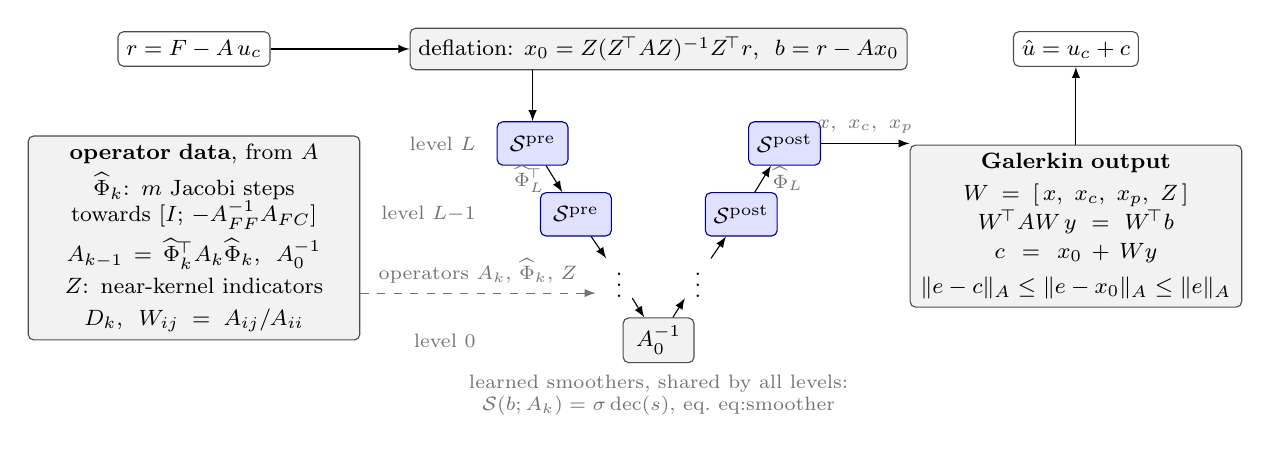
\begin{tikzpicture}[x=1cm, y=1cm, font=\footnotesize, >=latex,
  box/.style={draw=black!70, rounded corners=2pt, align=center, inner sep=3pt},
  op/.style={box, fill=black!5},
  learn/.style={box, fill=blue!12, draw=blue!60!black, minimum width=9mm, minimum height=5.5mm},
  lvl/.style={font=\scriptsize, text=black!55}]
% left: operator data
\node[box] (in) at (1.80,2.55) {$r = F - A\,u_c$};
\node[op, text width=40mm] (data) at (1.80,0.15) {\textbf{operator data}, from $A$\\[2pt]
  $\widehat\Phi_k$: $m$ Jacobi steps\\ towards $[I;\,-A_{FF}^{-1}A_{FC}]$\\[2pt]
  $A_{k-1}=\widehat\Phi_k^{\!\top}A_k\widehat\Phi_k$, \ $A_0^{-1}$\\[2pt]
  $Z$: near-kernel indicators\\[2pt] $D_k$, \ $W_{ij}=A_{ij}/A_{ii}$};
% middle: deflation and V-cycle
\node[op] (defl) at (7.70,2.55) {deflation: $x_0 = Z(Z^{\!\top}AZ)^{-1}Z^{\!\top}r$, \ $b = r - Ax_0$};
\node[learn] (s3) at (6.10,1.35) {$\mathcal{S}^{\mathrm{pre}}$};   \node[learn] (p3) at (9.30,1.35) {$\mathcal{S}^{\mathrm{post}}$};
\node[learn] (s2) at (6.65,0.45) {$\mathcal{S}^{\mathrm{pre}}$};  \node[learn] (p2) at (8.75,0.45) {$\mathcal{S}^{\mathrm{post}}$};
\node (s1) at (7.20,-0.35) {$\vdots$};                            \node (p1) at (8.20,-0.35) {$\vdots$};
\node[op, minimum width=9mm] (c0) at (7.70,-1.15) {$A_0^{-1}$};
\draw[->] (s3) -- node[left, lvl] {$\widehat\Phi_L^{\!\top}$} (s2);  \draw[->] (s2) -- (s1);  \draw[->] (s1) -- (c0);
\draw[->] (c0) -- (p1); \draw[->] (p1) -- (p2); \draw[->] (p2) -- node[right, lvl] {$\widehat\Phi_L$} (p3);
\node[lvl, anchor=east] at (5.50,1.35) {level $L$}; \node[lvl, anchor=east] at (5.50,0.45) {level $L{-}1$};
\node[lvl, anchor=east] at (5.50,-1.15) {level $0$};
\draw[->] (defl.south -| s3) -- (s3);
\node[lvl, align=center] at (7.70,-1.85) {learned smoothers, shared by all levels:\\ $\mathcal{S}(b;A_k) = \sigma\,\mathrm{dec}(s)$, eq.~\eqref{eq:smoother}};
% right: Galerkin output
\node[op, text width=40mm] (out) at (13.00,0.30) {\textbf{Galerkin output}\\[2pt]
  $W=[\,x,\ x_c,\ x_p,\ Z\,]$\\[1pt] $W^{\!\top}AW\,y = W^{\!\top}b$\\[1pt] $c = x_0 + Wy$\\[3pt]
  $\|e-c\|_A\le\|e-x_0\|_A\le\|e\|_A$};
\node[box] (res) at (13.00,2.55) {$\hat u = u_c + c$};
% connections
\draw[->] (in) -- (defl);
\draw[->, dashed, black!55] (data.east |- 0,-0.55) -- node[above, lvl] {operators $A_k$, $\widehat\Phi_k$, $Z$} (6.9,-0.55);
\draw[->] (p3.east) -- node[above, lvl] {$x,\ x_c,\ x_p$} (out.west |- p3.east);
\draw[->] (out) -- (res);
\end{tikzpicture}
 inside a figure environment.
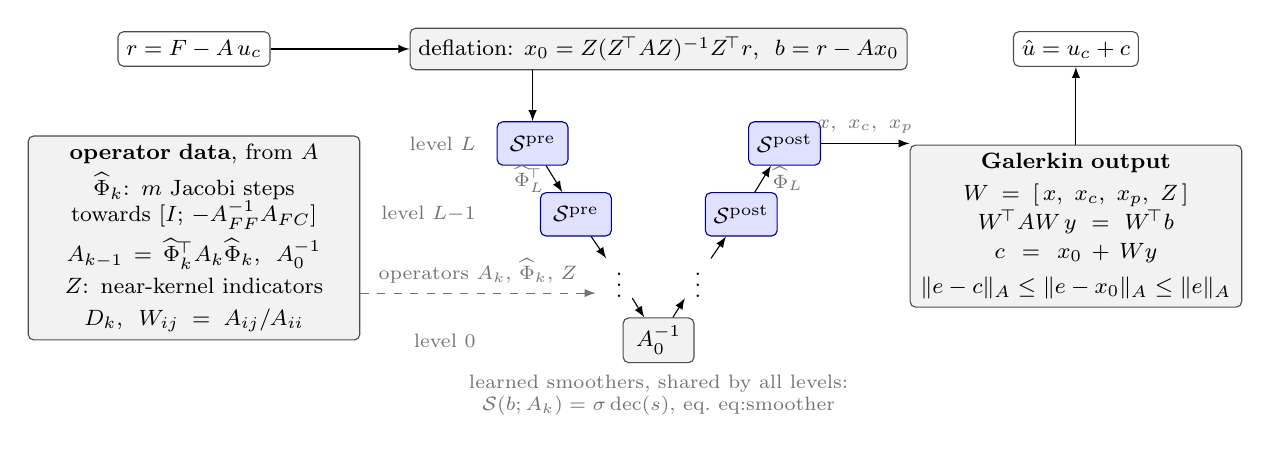
\begin{tikzpicture}[x=1cm, y=1cm, font=\footnotesize, >=latex,
  box/.style={draw=black!70, rounded corners=2pt, align=center, inner sep=3pt},
  op/.style={box, fill=black!5},
  learn/.style={box, fill=blue!12, draw=blue!60!black, minimum width=9mm, minimum height=5.5mm},
  lvl/.style={font=\scriptsize, text=black!55}]
% left: operator data
\node[box] (in) at (1.80,2.55) {$r = F - A\,u_c$};
\node[op, text width=40mm] (data) at (1.80,0.15) {\textbf{operator data}, from $A$\\[2pt]
  $\widehat\Phi_k$: $m$ Jacobi steps\\ towards $[I;\,-A_{FF}^{-1}A_{FC}]$\\[2pt]
  $A_{k-1}=\widehat\Phi_k^{\!\top}A_k\widehat\Phi_k$, \ $A_0^{-1}$\\[2pt]
  $Z$: near-kernel indicators\\[2pt] $D_k$, \ $W_{ij}=A_{ij}/A_{ii}$};
% middle: deflation and V-cycle
\node[op] (defl) at (7.70,2.55) {deflation: $x_0 = Z(Z^{\!\top}AZ)^{-1}Z^{\!\top}r$, \ $b = r - Ax_0$};
\node[learn] (s3) at (6.10,1.35) {$\mathcal{S}^{\mathrm{pre}}$};   \node[learn] (p3) at (9.30,1.35) {$\mathcal{S}^{\mathrm{post}}$};
\node[learn] (s2) at (6.65,0.45) {$\mathcal{S}^{\mathrm{pre}}$};  \node[learn] (p2) at (8.75,0.45) {$\mathcal{S}^{\mathrm{post}}$};
\node (s1) at (7.20,-0.35) {$\vdots$};                            \node (p1) at (8.20,-0.35) {$\vdots$};
\node[op, minimum width=9mm] (c0) at (7.70,-1.15) {$A_0^{-1}$};
\draw[->] (s3) -- node[left, lvl] {$\widehat\Phi_L^{\!\top}$} (s2);  \draw[->] (s2) -- (s1);  \draw[->] (s1) -- (c0);
\draw[->] (c0) -- (p1); \draw[->] (p1) -- (p2); \draw[->] (p2) -- node[right, lvl] {$\widehat\Phi_L$} (p3);
\node[lvl, anchor=east] at (5.50,1.35) {level $L$}; \node[lvl, anchor=east] at (5.50,0.45) {level $L{-}1$};
\node[lvl, anchor=east] at (5.50,-1.15) {level $0$};
\draw[->] (defl.south -| s3) -- (s3);
\node[lvl, align=center] at (7.70,-1.85) {learned smoothers, shared by all levels:\\ $\mathcal{S}(b;A_k) = \sigma\,\mathrm{dec}(s)$, eq.~\eqref{eq:smoother}};
% right: Galerkin output
\node[op, text width=40mm] (out) at (13.00,0.30) {\textbf{Galerkin output}\\[2pt]
  $W=[\,x,\ x_c,\ x_p,\ Z\,]$\\[1pt] $W^{\!\top}AW\,y = W^{\!\top}b$\\[1pt] $c = x_0 + Wy$\\[3pt]
  $\|e-c\|_A\le\|e-x_0\|_A\le\|e\|_A$};
\node[box] (res) at (13.00,2.55) {$\hat u = u_c + c$};
% connections
\draw[->] (in) -- (defl);
\draw[->, dashed, black!55] (data.east |- 0,-0.55) -- node[above, lvl] {operators $A_k$, $\widehat\Phi_k$, $Z$} (6.9,-0.55);
\draw[->] (p3.east) -- node[above, lvl] {$x,\ x_c,\ x_p$} (out.west |- p3.east);
\draw[->] (out) -- (res);
\end{tikzpicture}
 inside a figure environment.
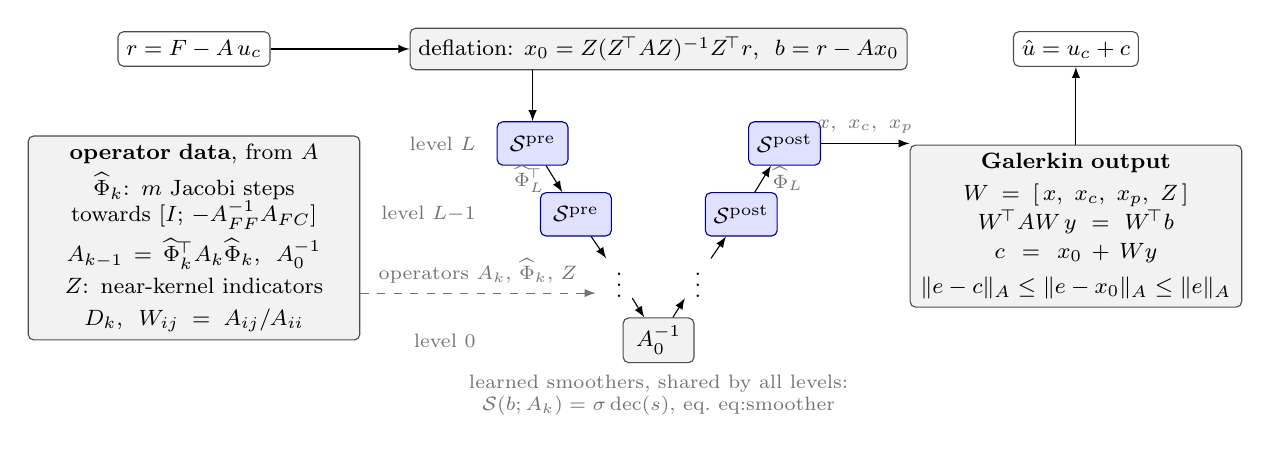
\begin{tikzpicture}[x=1cm, y=1cm, font=\footnotesize, >=latex,
  box/.style={draw=black!70, rounded corners=2pt, align=center, inner sep=3pt},
  op/.style={box, fill=black!5},
  learn/.style={box, fill=blue!12, draw=blue!60!black, minimum width=9mm, minimum height=5.5mm},
  lvl/.style={font=\scriptsize, text=black!55}]
% left: operator data
\node[box] (in) at (1.80,2.55) {$r = F - A\,u_c$};
\node[op, text width=40mm] (data) at (1.80,0.15) {\textbf{operator data}, from $A$\\[2pt]
  $\widehat\Phi_k$: $m$ Jacobi steps\\ towards $[I;\,-A_{FF}^{-1}A_{FC}]$\\[2pt]
  $A_{k-1}=\widehat\Phi_k^{\!\top}A_k\widehat\Phi_k$, \ $A_0^{-1}$\\[2pt]
  $Z$: near-kernel indicators\\[2pt] $D_k$, \ $W_{ij}=A_{ij}/A_{ii}$};
% middle: deflation and V-cycle
\node[op] (defl) at (7.70,2.55) {deflation: $x_0 = Z(Z^{\!\top}AZ)^{-1}Z^{\!\top}r$, \ $b = r - Ax_0$};
\node[learn] (s3) at (6.10,1.35) {$\mathcal{S}^{\mathrm{pre}}$};   \node[learn] (p3) at (9.30,1.35) {$\mathcal{S}^{\mathrm{post}}$};
\node[learn] (s2) at (6.65,0.45) {$\mathcal{S}^{\mathrm{pre}}$};  \node[learn] (p2) at (8.75,0.45) {$\mathcal{S}^{\mathrm{post}}$};
\node (s1) at (7.20,-0.35) {$\vdots$};                            \node (p1) at (8.20,-0.35) {$\vdots$};
\node[op, minimum width=9mm] (c0) at (7.70,-1.15) {$A_0^{-1}$};
\draw[->] (s3) -- node[left, lvl] {$\widehat\Phi_L^{\!\top}$} (s2);  \draw[->] (s2) -- (s1);  \draw[->] (s1) -- (c0);
\draw[->] (c0) -- (p1); \draw[->] (p1) -- (p2); \draw[->] (p2) -- node[right, lvl] {$\widehat\Phi_L$} (p3);
\node[lvl, anchor=east] at (5.50,1.35) {level $L$}; \node[lvl, anchor=east] at (5.50,0.45) {level $L{-}1$};
\node[lvl, anchor=east] at (5.50,-1.15) {level $0$};
\draw[->] (defl.south -| s3) -- (s3);
\node[lvl, align=center] at (7.70,-1.85) {learned smoothers, shared by all levels:\\ $\mathcal{S}(b;A_k) = \sigma\,\mathrm{dec}(s)$, eq.~\eqref{eq:smoother}};
% right: Galerkin output
\node[op, text width=40mm] (out) at (13.00,0.30) {\textbf{Galerkin output}\\[2pt]
  $W=[\,x,\ x_c,\ x_p,\ Z\,]$\\[1pt] $W^{\!\top}AW\,y = W^{\!\top}b$\\[1pt] $c = x_0 + Wy$\\[3pt]
  $\|e-c\|_A\le\|e-x_0\|_A\le\|e\|_A$};
\node[box] (res) at (13.00,2.55) {$\hat u = u_c + c$};
% connections
\draw[->] (in) -- (defl);
\draw[->, dashed, black!55] (data.east |- 0,-0.55) -- node[above, lvl] {operators $A_k$, $\widehat\Phi_k$, $Z$} (6.9,-0.55);
\draw[->] (p3.east) -- node[above, lvl] {$x,\ x_c,\ x_p$} (out.west |- p3.east);
\draw[->] (out) -- (res);
\end{tikzpicture}
 inside a figure environment.
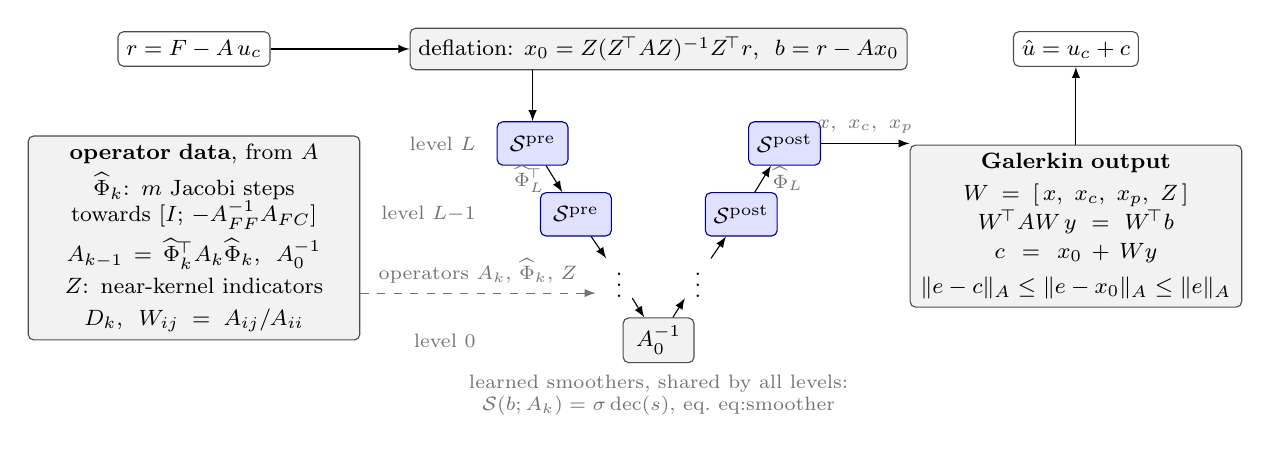
\begin{tikzpicture}[x=1cm, y=1cm, font=\footnotesize, >=latex,
  box/.style={draw=black!70, rounded corners=2pt, align=center, inner sep=3pt},
  op/.style={box, fill=black!5},
  learn/.style={box, fill=blue!12, draw=blue!60!black, minimum width=9mm, minimum height=5.5mm},
  lvl/.style={font=\scriptsize, text=black!55}]
% left: operator data
\node[box] (in) at (1.80,2.55) {$r = F - A\,u_c$};
\node[op, text width=40mm] (data) at (1.80,0.15) {\textbf{operator data}, from $A$\\[2pt]
  $\widehat\Phi_k$: $m$ Jacobi steps\\ towards $[I;\,-A_{FF}^{-1}A_{FC}]$\\[2pt]
  $A_{k-1}=\widehat\Phi_k^{\!\top}A_k\widehat\Phi_k$, \ $A_0^{-1}$\\[2pt]
  $Z$: near-kernel indicators\\[2pt] $D_k$, \ $W_{ij}=A_{ij}/A_{ii}$};
% middle: deflation and V-cycle
\node[op] (defl) at (7.70,2.55) {deflation: $x_0 = Z(Z^{\!\top}AZ)^{-1}Z^{\!\top}r$, \ $b = r - Ax_0$};
\node[learn] (s3) at (6.10,1.35) {$\mathcal{S}^{\mathrm{pre}}$};   \node[learn] (p3) at (9.30,1.35) {$\mathcal{S}^{\mathrm{post}}$};
\node[learn] (s2) at (6.65,0.45) {$\mathcal{S}^{\mathrm{pre}}$};  \node[learn] (p2) at (8.75,0.45) {$\mathcal{S}^{\mathrm{post}}$};
\node (s1) at (7.20,-0.35) {$\vdots$};                            \node (p1) at (8.20,-0.35) {$\vdots$};
\node[op, minimum width=9mm] (c0) at (7.70,-1.15) {$A_0^{-1}$};
\draw[->] (s3) -- node[left, lvl] {$\widehat\Phi_L^{\!\top}$} (s2);  \draw[->] (s2) -- (s1);  \draw[->] (s1) -- (c0);
\draw[->] (c0) -- (p1); \draw[->] (p1) -- (p2); \draw[->] (p2) -- node[right, lvl] {$\widehat\Phi_L$} (p3);
\node[lvl, anchor=east] at (5.50,1.35) {level $L$}; \node[lvl, anchor=east] at (5.50,0.45) {level $L{-}1$};
\node[lvl, anchor=east] at (5.50,-1.15) {level $0$};
\draw[->] (defl.south -| s3) -- (s3);
\node[lvl, align=center] at (7.70,-1.85) {learned smoothers, shared by all levels:\\ $\mathcal{S}(b;A_k) = \sigma\,\mathrm{dec}(s)$, eq.~\eqref{eq:smoother}};
% right: Galerkin output
\node[op, text width=40mm] (out) at (13.00,0.30) {\textbf{Galerkin output}\\[2pt]
  $W=[\,x,\ x_c,\ x_p,\ Z\,]$\\[1pt] $W^{\!\top}AW\,y = W^{\!\top}b$\\[1pt] $c = x_0 + Wy$\\[3pt]
  $\|e-c\|_A\le\|e-x_0\|_A\le\|e\|_A$};
\node[box] (res) at (13.00,2.55) {$\hat u = u_c + c$};
% connections
\draw[->] (in) -- (defl);
\draw[->, dashed, black!55] (data.east |- 0,-0.55) -- node[above, lvl] {operators $A_k$, $\widehat\Phi_k$, $Z$} (6.9,-0.55);
\draw[->] (p3.east) -- node[above, lvl] {$x,\ x_c,\ x_p$} (out.west |- p3.east);
\draw[->] (out) -- (res);
\end{tikzpicture}
